%!TEX root = ../template.tex
%%%%%%%%%%%%%%%%%%%%%%%%%%%%%%%%%%%%%%%%%%%%%%%%%%%%%%%%%%%%%%%%%%%%
%% chapter4.tex
%% NOVA thesis document file
%%
%% Chapter with lots of dummy text
%%%%%%%%%%%%%%%%%%%%%%%%%%%%%%%%%%%%%%%%%%%%%%%%%%%%%%%%%%%%%%%%%%%%

\typeout{NT FILE chapter4.tex}%

\chapter{Experiments with Generative AI techniques and tools}
\label{cha:ExperimentsGenerativeAI}

This chapter reports the preliminary experiments conducted to configure an automated pipeline that generates UML class diagrams from natural-language system descriptions. We compare prompt-engineering strategies and large language models (LLMs), and we evaluate Retrieval-Augmented Generation (RAG) settings to identify the combination that best supports this task. We also test a self-refinement loop in which the model critiques and revises its own output to improve quality. The chapter is organised as follows: Section \ref{sec:ExperimentPromptModel} examines prompt techniques and model choice; Section \ref{sec:rag_experiments} evaluates a RAG-based approach; and Section~\ref{sec:selfRefinementApproach} investigates self-refinement.

\section{Experiments with prompt techniques and different LLM models}
\label{sec:ExperimentPromptModel}
To probe how prompt engineering and model choice interact when converting natural‐language requirements into UML class diagrams, we conducted a controlled experiment structured according to the setup represented in Figure ~\ref{fig:experimentalSetup}. The experiment was centred on a single, medium-sized specification drawn from the dataset of Daniele De Bari et al. \cite{DatasetDeBari2024}. We decided to use this dataset because besides having the system description and the associated benchmark class diagram it also has a class diagram that was created by a human. By having this two class diagram it allows us to have a deeper evaluation of the generated diagrams.
Listing~\ref{lst:system_description} shows the excerpt; it contains multiple actors, artefacts, and life-cycle constraints—enough complexity to exercise class identification, attribute extraction, and relationship mapping.

\begin{lstlisting}[caption={System Description}, label={lst:system_description}, float = htb]
A project manager uses the project management system to manage a project. The project manager leads a team to execute the project within the project's start and end dates.
Once a project is created in the project management system, a manager may initiate and later terminate the project due to its completion or for some other reason.
As input, a project uses requirements. As output, a project produces a system (or part of a system). The requirements and system are work products: things that are created, used, updated, and elaborated on throughout a project.
Every work product has a description, is of some percent complete throughout the effort, and may be validated.
However, validation is dependent on the type of work product. For example, the requirements are validated with users in workshops, and the system is validated by being tested against the requirements.
Furthermore, requirements may be published using various types of media, including on an intranet or in paper form; and systems may be deployed onto specific platforms.
\end{lstlisting}

As it can be seen in Figure ~\ref{fig:experimentalSetup}, after the dataset was defined, we designed an experiment to systematically evaluate the impact of different prompt strategies and model choices. The experimental setup is described below.

\begin{figure}[htbp]
    \centering
    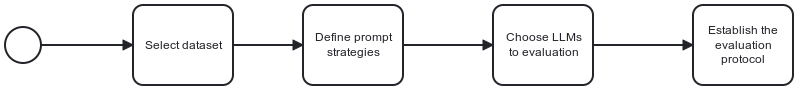
\includegraphics[width=0.6\linewidth]{Chapters/Figures/Prompt_expirement.png} % Adjust width or use height
    \caption{ Experimental setup for prompt techniques and LLMs tests }
    \label{fig:experimentalSetup}
\end{figure}

\paragraph{Define prompt strategies}
Each model was queried under three canonical strategies:

\begin{enumerate}
\item \textbf{Zero-shot} – task instruction only;
\item \textbf{Few-shot} – three worked examples followed by the target specification;
\item \textbf{Chain-of-thought Few-shot (CoT)} – the few-shot template augmented with an explicit, step-by-step reasoning scaffold.
\end{enumerate}
The prompts used for testing can be found in the Appendix ~\ref{app:prompt_testing}.

\paragraph{Choose LLMs to Evaluate}
We considered five commercially hosted models that can be accessed without a local GPU:

\begin{enumerate}
    \item ChatGPT-4o;
    \item Claude Sonnet 4;
    \item Deepshek XL;
    \item Gemini 2.5 Flash; 
    \item Grok 1.5;
\end{enumerate}

Several open-source models (Mistral 7B, Qwen 7B, Falcon 7B) were piloted but discarded because the presented results were weak. Some generated PlantUML code had syntax errors that did not allow to compile, others were not able to generate PlantUML code. 
Besides this, when we used few-shot prompting, some models generated class diagrams not related with the system description but related with the examples presented in the prompt.
We still tried using opensource models with more parameters, although they had better results, they were significantly worse then those obtain with the commercial models. 
Therefore, do to weak results and hardware limitations to run powerfull open source models we end up discarding opens ource for this tests.

\paragraph{Evaluation protocol}

The generated diagrams were assessed along three complementary axes:

\begin{enumerate}
    \item \textbf{Structure.}
        We compared each diagram to the ground-truth model via a confusion matrix over classes, attributes, and relationships, computing precision, recall, and $F_1$.
    \item \textbf{Semantic and pragmatic adequacy.}
        We adopted G-Eval \cite{liu2023gevalnlgevaluationusing} with Llama-3 as the grader, requesting two rubric items: \emph{semantic fidelity} (correctness and completeness of domain concepts) and \emph{pragmatic usefulness} (clarity, UML idioms and multiplicities).
    \item \textbf{Lexical overlap.}
        ROUGE-L recall \cite{lin-2004-rouge} was computed between the generated PlantUML and the reference code. Although surface-oriented, ROUGE helps detect omissions that structural matching alone may miss (e.g., lost attributes).
\end{enumerate}
\subsection{Results and Discussion}

Figures \ref{fig:combined_metrics} and \ref{fig:overall_metrics} visualise the outcome. We analyze the main findings below.

\paragraph{Prompt strategy effects.}
CoT delivers the highest mean G-Eval and the strongest recall, confirming that an explicit reasoning trace helps models surface low-salience entities such as \textit{WorkProduct}. However, its ROUGE score lags behind few-shot because the additional prose dilutes lexical overlap with the gold PlantUML.
Few-shot, in contrast, attains the best ROUGE and the second-best recall, suggesting that concise demonstrations strike a balance between coverage and verbosity. Zero-shot performs adequately on ChatGPT-4o but drops in both recall and G-Eval for the remaining models.

\paragraph{Model behaviour}
\begin{itemize}
    \item \textbf{Claude Sonnet 4} consistently tops the G-Eval table and ranks second in structural recall, making it the most balanced performer.
    \item \textbf{Deepseek} yields the highest recall and~$F_1$, although with slightly lower G-Eval. This is an indicator that it enumerates more elements but produces output with less refinement compared to Claude.
    \item \textbf{ChatGPT-4o} excels in zero-shot but gains little from additional prompting.
    \item \textbf{Gemini 2.5 Flash} shows moderate scores across metrics, hampered by occasional length truncation in CoT mode.
    \item \textbf{Grok 1.5} underperforms structurally and, in CoT mode, returned an image instead of code, highlighting alignment gaps for specialised tasks.
\end{itemize}


\begin{figure}[htbp]
    \centering
    
    \subfloat[Recall of each LLM model per prompt technique]{%
        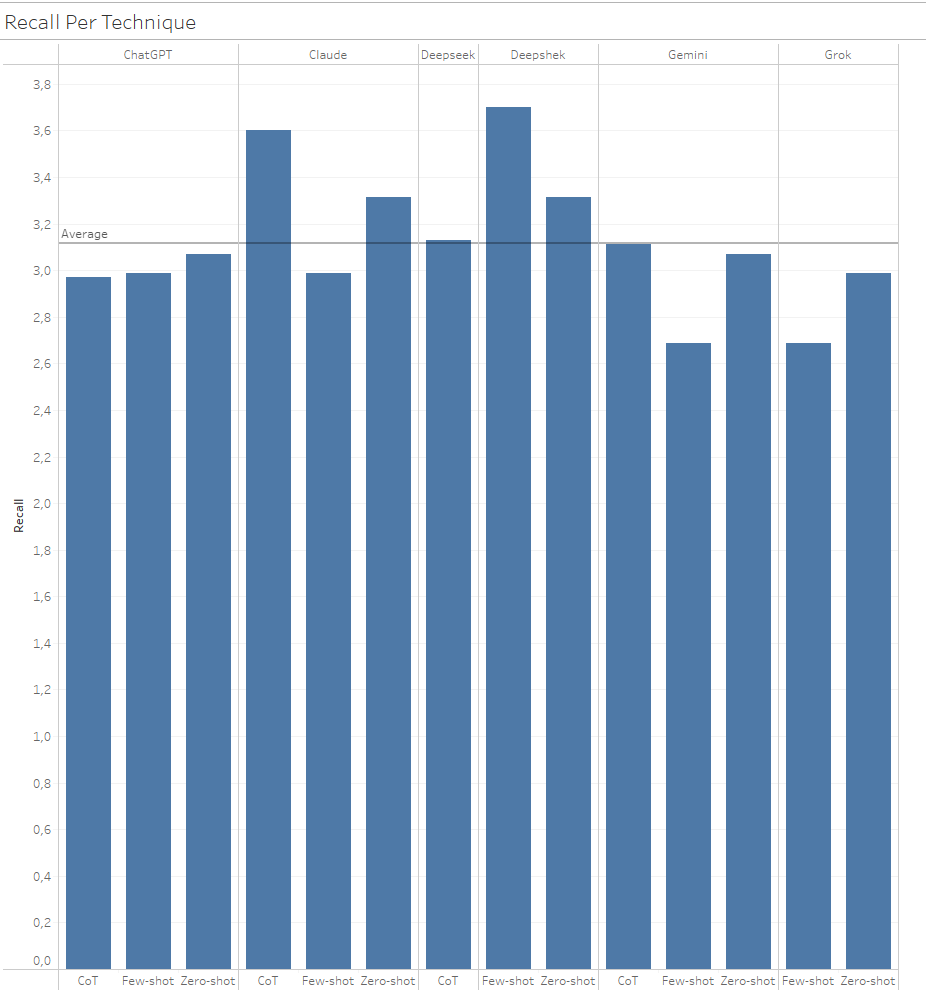
\includegraphics[width=0.6\textwidth, height = 0.3\textheight]{Chapters/Figures/RecallTechniques.png}
        \label{fig:RecalTechniques}
    }\\[0.3cm]
    
    \subfloat[G-Eval of each LLM model per prompt technique]{%
        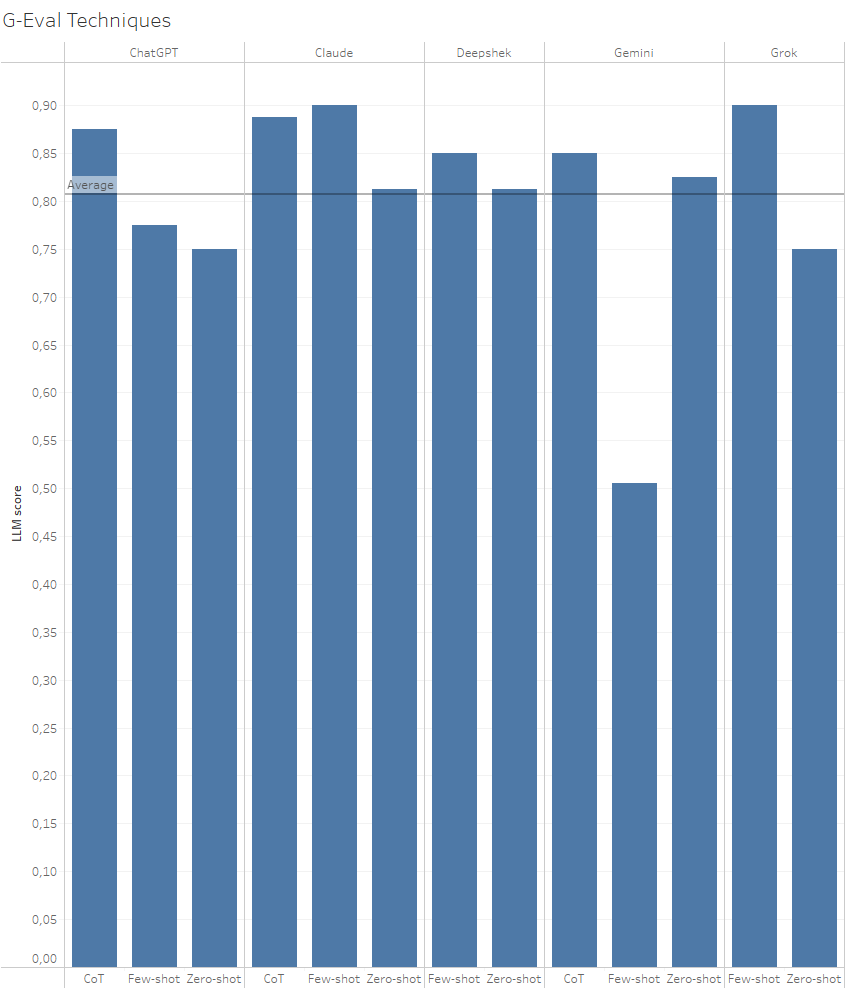
\includegraphics[width=0.6\textwidth, height = 0.3\textheight]{Chapters/Figures/G-evalTechniques.png}
        \label{fig:gevalTechniques}
    }\\[0.3cm]
    
    \subfloat[ROUGE of each LLM model per prompt technique]{%
        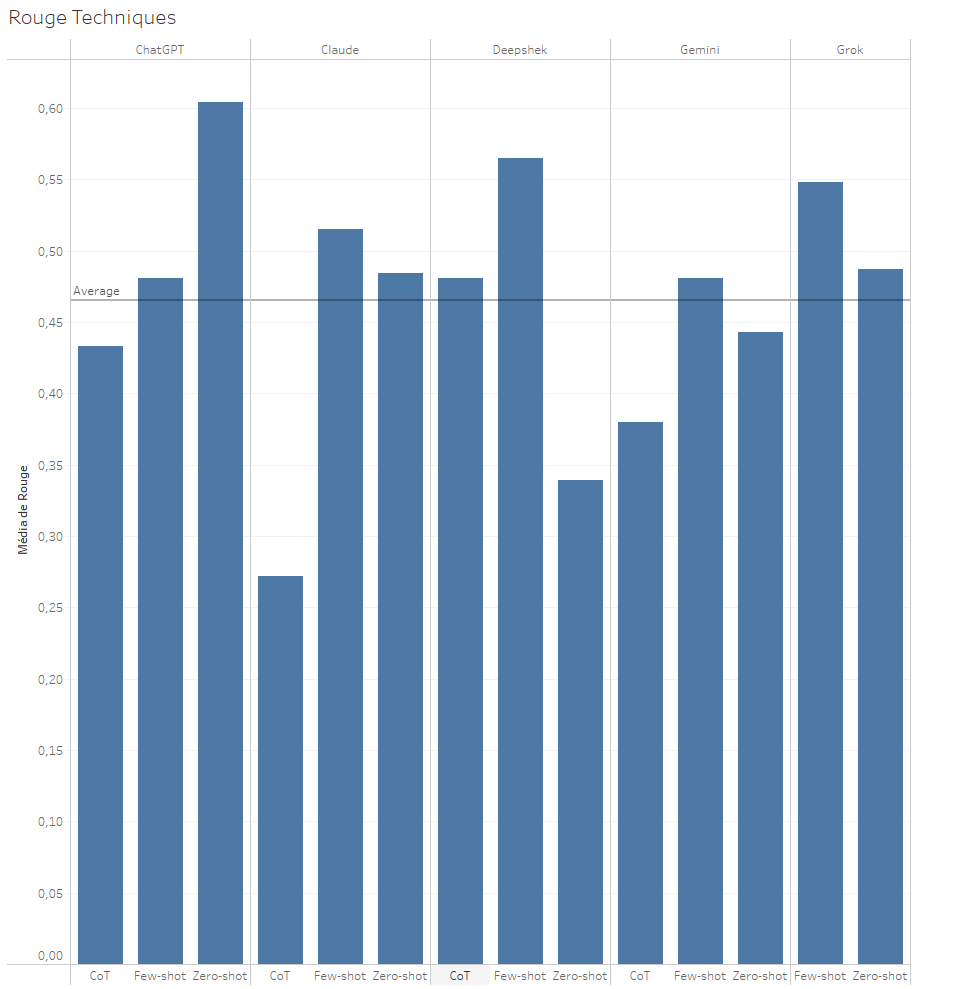
\includegraphics[width=0.6\textwidth, height = 0.3\textheight]{Chapters/Figures/RougeTechniques.png}
        \label{fig:rouge}
    }
    
    \caption{Evaluation results across prompting strategies and models.}
    \label{fig:combined_metrics}
\end{figure}

\begin{figure}[htbp]
    \centering
    
    \subfloat[Recall of each LLM model overall]{%
        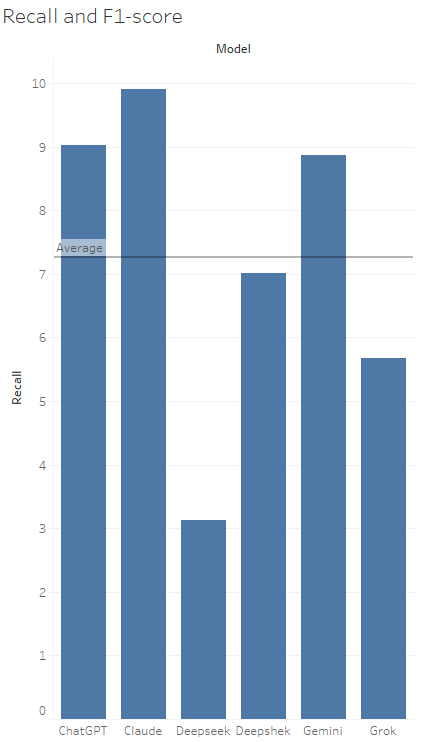
\includegraphics[width=0.6\textwidth, height = 0.3\textheight]{Chapters/Figures/RecallModel.png}
        \label{fig:RecalOverall}
    }\\[0.3cm]
    
    \subfloat[G-Eval of each LLM model overall]{%
        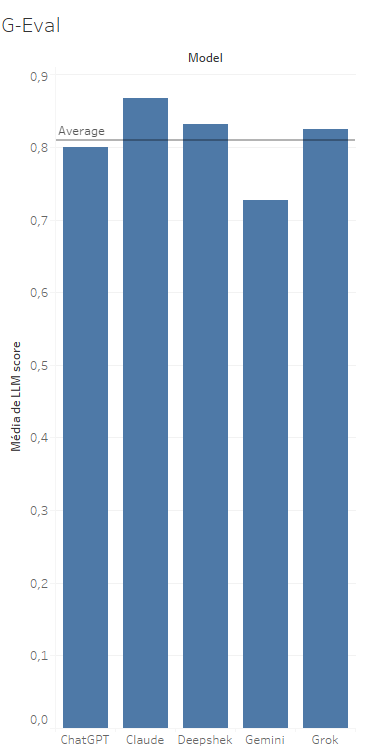
\includegraphics[width=0.6\textwidth, height = 0.3\textheight]{Chapters/Figures/G-evalModel.png}
        \label{fig:gevalOverall}
    }\\[0.3cm]
    
    \subfloat[ROUGE of each LLM model overall]{%
        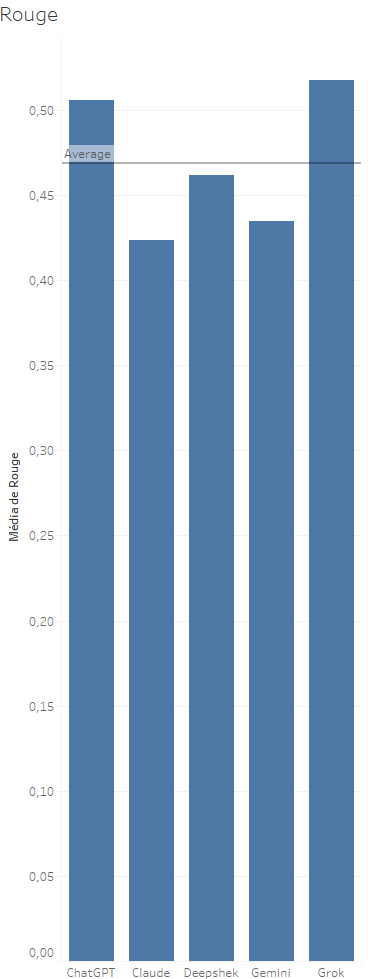
\includegraphics[width=0.6\textwidth, height = 0.3\textheight]{Chapters/Figures/Rouge.png}
        \label{fig:rougeOverall}
    }
    
    \caption{Evaluation results across prompting strategies and models.}
    \label{fig:overall_metrics}
\end{figure}



\section{Experiments with a Retrieval-Augmented Generation (RAG) Tool}
\label{sec:rag_experiments}
To further understand if implementing a RAG system would be beneficial for generation of class diagrams we conducted experiments using the new google tool, NotebookLM. \footnote{Formerly “Project Tailwind,” an AI-assisted research and note-taking environment released by Google Labs.}
NotebookLM grounds its responses in a user-supplied document collection, thereby enabling context-aware retrieval during generation \cite{martin2023notebooklm}.  


\subsection{Experimental Setup}

To conduct this experiment  we configured a notebook by adding the following documents.
Aiming to simulate the reference material available to a professional modeller:
\begin{enumerate}
    \item Buku-learning UML 2.0 – A pedagogical guide to UML concepts.
    \item OMG UML specification – The official UML language specification.
    \item PlantUML reference guide – Syntax and rendering documentation for PlantUML.
    \item Examples from the UML modeling dataset – Simulating models created in previous projects
\end{enumerate}

An important limitation found is that the NotebookLM imposes constraints on the number of tokens, limiting the possibilities of using prompting engineering. Therefore, we were only able to use zero-shot prompt supported by RAG context.

We directly prompt the zero shot prompt used in the previous experiment but we deleted the last part where is the information about PlantUML syntax due to token limitations and the fact that this guidance had already been included in the database.
Looking at the result we could see that a class diagram was no different from the previously generated in the first experiment. Having similar results to the one presented by the Google model (Gemini).

To improve the quality of the generated diagrams, we rewrote the zero-shot prompt so that it was better suited for use in a RAG tool. The revised prompt included an explicit reference to RAG, direct instructions to leverage the knowledge base, and a more structured format to facilitate parsing.

This adaptation produced better results than the original prompt. The second diagram not only identified an additional relationship absent from the first but also aligned more closely with the ground truth benchmark. 
However, in both cases the models struggled to capture all the necessary attributes (Prompt~\ref{lst:zero_shot_adapted}). In particular, while the first diagram incorrectly represented the attributes Platform and MediaType as separate classes—reducing legibility—the second omitted these elements entirely, as shown in Figure~\ref{fig:classDiagrams_NotebookLM}.

\begin{lstlisting}[caption={Adapted Zero-shot prompt}, label={lst:zero_shot_adapted}]
You are an experienced software engineer specializing in UML modeling. Based on the UML specifications, PlantUML documentation, and modeling examples available in your knowledge base, create a class diagram for a project management system.

**System Requirements:**
The project manager leads a team to execute projects within defined start and end dates. Once created in the system, a manager may initiate and later terminate projects due to completion or other reasons. The team executes the project using requirements as input to produce a system as output.

Requirements and systems are work products with descriptions, completion percentages, and validation capabilities. Requirements are validated through user workshops, while systems are validated by testing against requirements. Requirements may be published via various media (intranet, paper), and systems may be deployed on specific platforms.

**Instructions:**
- Follow UML class diagram principles from your knowledge base
- Use PlantUML syntax as documented in your references
- Generate clean PlantUML code without comments or references
- Focus on: classes, attributes, methods, relationships, and multiplicities
- Ensure all entities mentioned in requirements are properly modeled

Output only valid PlantUML code.
\end{lstlisting}

\begin{figure}[htb]
  \centering

  \subfloat[Zero-shot prompt\label{fig:nb_left}]{
    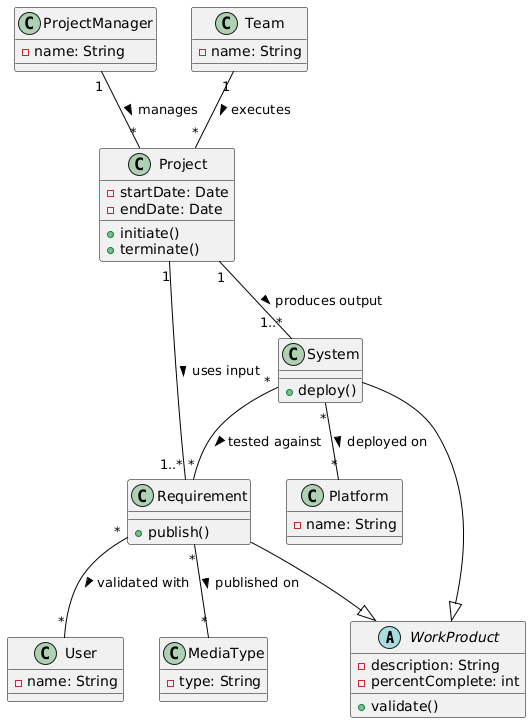
\includegraphics[width=0.5\textwidth,height=0.30\textheight,keepaspectratio]
      {Chapters/Figures/ClassDiagram_SystemDescription.png}}
  \hfill
  \subfloat[Zero-shot prompt adapted for RAG\label{fig:nb_right}]{
    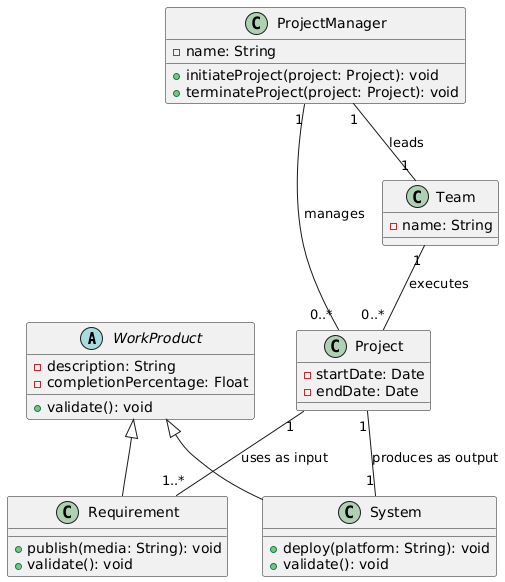
\includegraphics[width=0.5\textwidth,height=0.30\textheight,keepaspectratio]
      {Chapters/Figures/ClassDiagram_SecondPrompt.png}}

  \vspace{0.4em}

 

  \caption{Different class diagrams generated using NotebookLM compared to the ground truth.}
  \label{fig:classDiagrams_NotebookLM}
\end{figure}


\subsection{Results and Discussion}
Comparing to the results obtained in the first experiment we can see that the generated class diagram with the adapted prompt is the most close to the ground truth. Obtaining the best precision, recall, and F1-score in all elements of the class diagram besides attributes.
This results suggest that RAG can be beneficial to generate class diagrams from system descriptions.

\section{Experimenting Self-improving}
An emerging technique in the field of generative artificial intelligence is self-refinement, a process wherein LLMs iteratively improve their own outputs by generating feedback and revising responses without human intervention. This paradigm mirrors the structure of human-in-the-loop feedback systems but replaces the human evaluator with the model itself, thereby enabling a form of autonomous self-improvement.
Madaan et al. (2023) formalized this approach through the Self-Refine framework, demonstrating that an LLM can act simultaneously as generator, critic, and refiner via prompt chaining. Their experiments across diverse tasks—including mathematical reasoning and open-domain question answering—revealed an average absolute improvement of approximately 20\% in performance compared to traditional one-shot generation methods \cite{NEURIPS2023_91edff07}.
A key advantage of this technique is its ability to enhance model performance entirely at inference time, leveraging prompt engineering and in-context feedback, without resorting to computationally expensive fine-tuning or additional training \cite{NEURIPS2023_91edff07}. This makes it particularly suitable for our setting with limited computational resources. 
Motivated by these promising results, we conducted a series of experiments to assess whether self-refinement could enhance the performance of our own generative system. Specifically, we aimed to explore the impact of iterative self-evaluation and refinement on the quality and accuracy of generated outputs within our use case.

\subsection{Experimental Setup}
To implement the self-refinement methodology, we developed a Python-based experimental pipeline that leverages the Anthropic Claude API to simulate a reflective reasoning loop. This loop enables a generative model to not only produce UML class diagrams from natural language system descriptions but also to autonomously evaluate and iteratively improve its own output based on structured critique.
The Anthropic Claude model was selected due to its strong performance in prior experiments (see Section~\ref{sec:ExperimentPromptModel}) and its free-tier access, which allowed us to execute multiple inference rounds without incurring computational or financial overhead. These practical and performance-based criteria rendered Claude an appropriate model for experimentation in resource-constrained environments.
The self-refinement loop is implemented as a three-step iterative process capped at a maximum of three iterations. The sequence is as follows:

\begin{enumerate}
    \item Initial Generation: Firstly, the system uses a chain-of-thought (CoT) prompt—previously evaluated and available in Appendix~\ref{app:prompt_testing}— to generate the class diagram based system description. This response constitutes the starting output to be refined.

    \item Self-Evaluation: The generated diagram is passed to a structured evaluation function (see Prompt~\ref{lst:self_evaluate}) which queries the Claude model to assess the quality of the diagram across four rigorously defined dimensions: UML completeness, UML syntax and quality, requirement coverage, and clarity and pragmatics. Each dimension is weighted, and an overall evaluation score is computed. The response includes both scalar scores and detailed natural language feedback in JSON format, ensuring both interpretability and machine-readability.

    \item Self-Improvement: If the initial output does not meet the quality threshold—defined or higher a refinement step is triggered. In this step, the previously generated diagram, the system description, and the evaluation feedback are incorporated into an improvement prompt (Prompt~\ref{lst:self_improve}). This prompt instructs the model to revise the class diagram to resolve the identified issues and implement the suggested enhancements. The revised output is then subjected to a new round of self-evaluation.
\end{enumerate}

\begin{lstlisting}[caption={Self improve}, label={lst:self_improve}, float = htb]
 #SYSTEM PROMPT
    You are an expert UML software architect tasked with improving a PlantUML class diagram based on specific feedback and evaluation criteria.

        ## Your Task
        Analyze the provided feedback and systematically improve the class diagram to address all identified issues while maintaining the original system requirements.

        ## Improvement Guidelines

        ### 1. UML Completeness Improvements
        - Add missing classes, attributes, or methods identified in feedback
        - Ensure all entities from system description are represented
        - Include proper visibility modifiers (-, +, #)
        - Add missing relationships and associations

        ### 2. UML Quality Enhancements
        - Fix naming convention issues (PascalCase for classes, camelCase for attributes/methods)
        - Correct relationship types (association, aggregation, composition, inheritance)
        - Improve multiplicity specifications
        - Enhance method signatures with proper parameters and return types

        ### 3. Requirement Coverage Improvements
        - Map every requirement explicitly mentioned in system description
        - Ensure behavioral aspects are captured through appropriate methods
        - Add missing domain-specific attributes and operations
        - Include all stated constraints and business rules

        ### 4. Clarity & Pragmatic Improvements
        - Improve relationship labels for better understanding
        - Organize classes logically (group related classes)
        - Add stereotypes where appropriate (<<interface>>, <<abstract>>, etc.)
        - Ensure proper abstraction levels

        ## Output Instructions
        1. Provide the complete improved PlantUML diagram
        2. Start with @startuml and end with @enduml
        3. Include all improvements addressing the feedback
        4. Maintain syntactic correctness
        5. Ensure the diagram is more comprehensive than the original

        ## Critical Requirements
        - Address ALL issues mentioned in the feedback
        - Implement ALL recommendations provided
        - Ensure the improved diagram scores higher in all evaluation dimensions
        - Maintain or enhance requirement coverage
        - Keep PlantUML syntax error-free

        ##Important Note: 
        - Follow strictly the System Description. Keep the diagram simple and direct.

    USER PROMPT 
    Improve the following PlantUML class diagram based on the following feedback:      
            ## Current PlantUML Class Diagram
            {current_response}

            ## Detailed Feedback Analysis
            {json.dumps(feedback.get('feedback', ''), indent=2)}

            ## Specific Issues to Address
            {chr(10).join(f"- {issue}" for issue in feedback.get('issues', []))}

            ## Recommendations to Implement
            {chr(10).join(f"- {rec}" for rec in feedback.get('recommendations', []))}   
\end{lstlisting}

\begin{lstlisting}[caption={Self evaluation}, label={lst:self_evaluate}, float = htb]
#SYSTEM PROMPT 
You are an expert UML evaluator and software engineering reviewer with deep expertise in system analysis and design quality assessment. Your task is to comprehensively evaluate a UML class diagram against system requirements using rigorous academic and industry standards.

        ## Evaluation Framework

        Assess the class diagram across these four critical dimensions:

        ### 1. UML Completeness (25% weight)
        **Criteria:**
        - All relevant classes identified and included
        - Complete set of attributes for each class with appropriate types
        - Comprehensive method signatures with parameters and return types
        - Proper visibility modifiers (-, +, #) applied consistently
        - All necessary relationships present (associations, inheritance, dependencies)

        **Scoring:**
        - 0.9-1.0: All elements present, comprehensive coverage
        - 0.7-0.8: Minor omissions, mostly complete
        - 0.5-0.6: Several missing elements
        - 0.3-0.4: Major gaps in completeness
        - 0.0-0.2: Severely incomplete

        ### 2. UML Quality (25% weight)
        **Criteria:**
        - Correct UML syntax and notation
        - Proper relationship types (composition vs aggregation vs association)
        - Accurate multiplicity specifications
        - Consistent naming conventions (PascalCase classes, camelCase attributes/methods)
        - Appropriate use of abstract classes and interfaces
        - Proper encapsulation and information hiding

        **Scoring:**
        - 0.9-1.0: Excellent quality, best practices followed
        - 0.7-0.8: Good quality with minor issues
        - 0.5-0.6: Adequate quality, some problems
        - 0.3-0.4: Poor quality, multiple issues
        - 0.0-0.2: Very poor quality, major problems

        ### 3. Requirement Coverage (30% weight)
        **Criteria:**
        - Every entity mentioned in requirements is modeled
        - All relationships described in requirements are captured
        - Business rules and constraints are represented
        - Behavioral aspects are included through appropriate methods
        - Domain-specific terminology is preserved
        - System boundaries and scope are respected

        **Scoring:**
        - 0.9-1.0: Complete requirement coverage
        - 0.7-0.8: Most requirements covered, minor gaps
        - 0.5-0.6: Adequate coverage, some missing aspects
        - 0.3-0.4: Poor coverage, major requirements missing
        - 0.0-0.2: Very poor coverage, most requirements ignored

        ### 4. Clarity & Pragmatics (20% weight)
        **Criteria:**
        - Diagram is understandable to technical stakeholders
        - Logical organization and grouping of classes
        - Meaningful relationship labels and role names
        - Appropriate level of abstraction
        - Clear separation of concerns
        - Professional presentation and layout

        **Scoring:**
        - 0.9-1.0: Exceptionally clear and well-organized
        - 0.7-0.8: Clear and understandable
        - 0.5-0.6: Reasonably clear, some confusion possible
        - 0.3-0.4: Unclear in several areas
        - 0.0-0.2: Very unclear, difficult to understand

        ## Evaluation Instructions

        1. **Systematic Analysis**: Examine each dimension thoroughly
        2. **Evidence-Based Scoring**: Provide specific examples for scores
        3. **Detailed Issues**: List concrete problems with specific locations
        4. **Actionable Recommendations**: Provide implementable improvements
        5. **Comprehensive Assessment**: Consider the diagram as a whole system model

        ## Required Output Format

        Return ONLY a valid JSON object with this exact structure:

        ```json
        {{
            "uml_completeness_score": <float 0.0-1.0>,
            "uml_quality_score": <float 0.0-1.0>,
            "requirement_coverage_score": <float 0.0-1.0>,
            "pragmatic_clarity_score": <float 0.0-1.0>,
            "overall_score": <float 0.0-1.0>,
            "detailed_analysis": {{
                "completeness_details": "<specific analysis of what's missing or present>",
                "quality_details": "<analysis of UML syntax, conventions, and design quality>",
                "coverage_details": "<analysis of how well requirements are captured>",
                "clarity_details": "<analysis of diagram understandability and organization>"
            }},
            "issues": [
                "<specific issue 1 with location/context>",
                "<specific issue 2 with location/context>",
                "<specific issue 3 with location/context>"
            ],
            "recommendations": [
                "<actionable recommendation 1>",
                "<actionable recommendation 2>",
                "<actionable recommendation 3>"
            ],
            "strengths": [
                "<identified strength 1>",
                "<identified strength 2>"
            ]
        }}
        ```
        If there is no issues or recommendations, you can return an empty array for those fields.
        Calculate the overall_score as: (uml_completeness_score * 0.25) + (uml_quality_score * 0.25) + (requirement_coverage_score * 0.30) + (pragmatic_clarity_score * 0.20)"""
#USER PROMPT 
    Evaluate the following PlantUML class diagram based on the following system descripting:

        **System Description**
        {system_description}

        **PlantUML class diagram**
        {response}
        Base your response exclusively on the system description and in the UML principles
\end{lstlisting}

This loop continues iteratively until either a satisfactory score is achieved or the maximum number of iterations is reached.
To support transparency and replicability, the pipeline maintains a persistent logging system that records all iterations, feedback evaluations, and diagram versions. Additionally, a structured feedback\_history data structure is maintained, which stores for each iteration: (i) the feedback JSON object, (ii) the corresponding PlantUML diagram, and (iii) the iteration number. This facilitates post-hoc analysis and supports visual inspection of improvement trends.
Overall, this experimental design allows us to rigorously test whether self-reflective generation—achieved entirely through inference-time prompting—can lead to substantial and consistent improvements in UML modeling tasks. The design aligns with emerging research advocating for \textit{low-cost, feedback-driven refinement frameworks} (e.g., Madaan et al., 2023), which offer a viable alternative to expensive fine-tuning or supervised retraining in downstream applications.

To decide when to stop the loop, we used a threshold. To know which is the best threshold that fits our goal the better we run the script with different thresholds ranging from 0.7 to 0.95. 
As it can be seen in the Figure ~\ref{fig:thresholdTest}, we recorded the average score, average iterations done and the standard deviation of the score. This way we can analyse the effort needed to achieve a certain threshold and the stability of those scores.
The thresholds 0.75 to 0.85 have high average scores and low iteration scores. The threshold 0.85 seems to be more stable.
The threshold 0.9 achieves the highest scores but at the cost of the number of iterations. Also, it has the highest standard deviation which indicates that is less predictable in terms of performance.
The last threshold has slightly worst score then the previous threshold but with a higher number of iterations. Although is more stable then 0.9 threshold.

Looking at this results we end up deciding to use 0.85 because it overs the best cost-benefit ratio.
\begin{figure}[htbp]
    \centering
    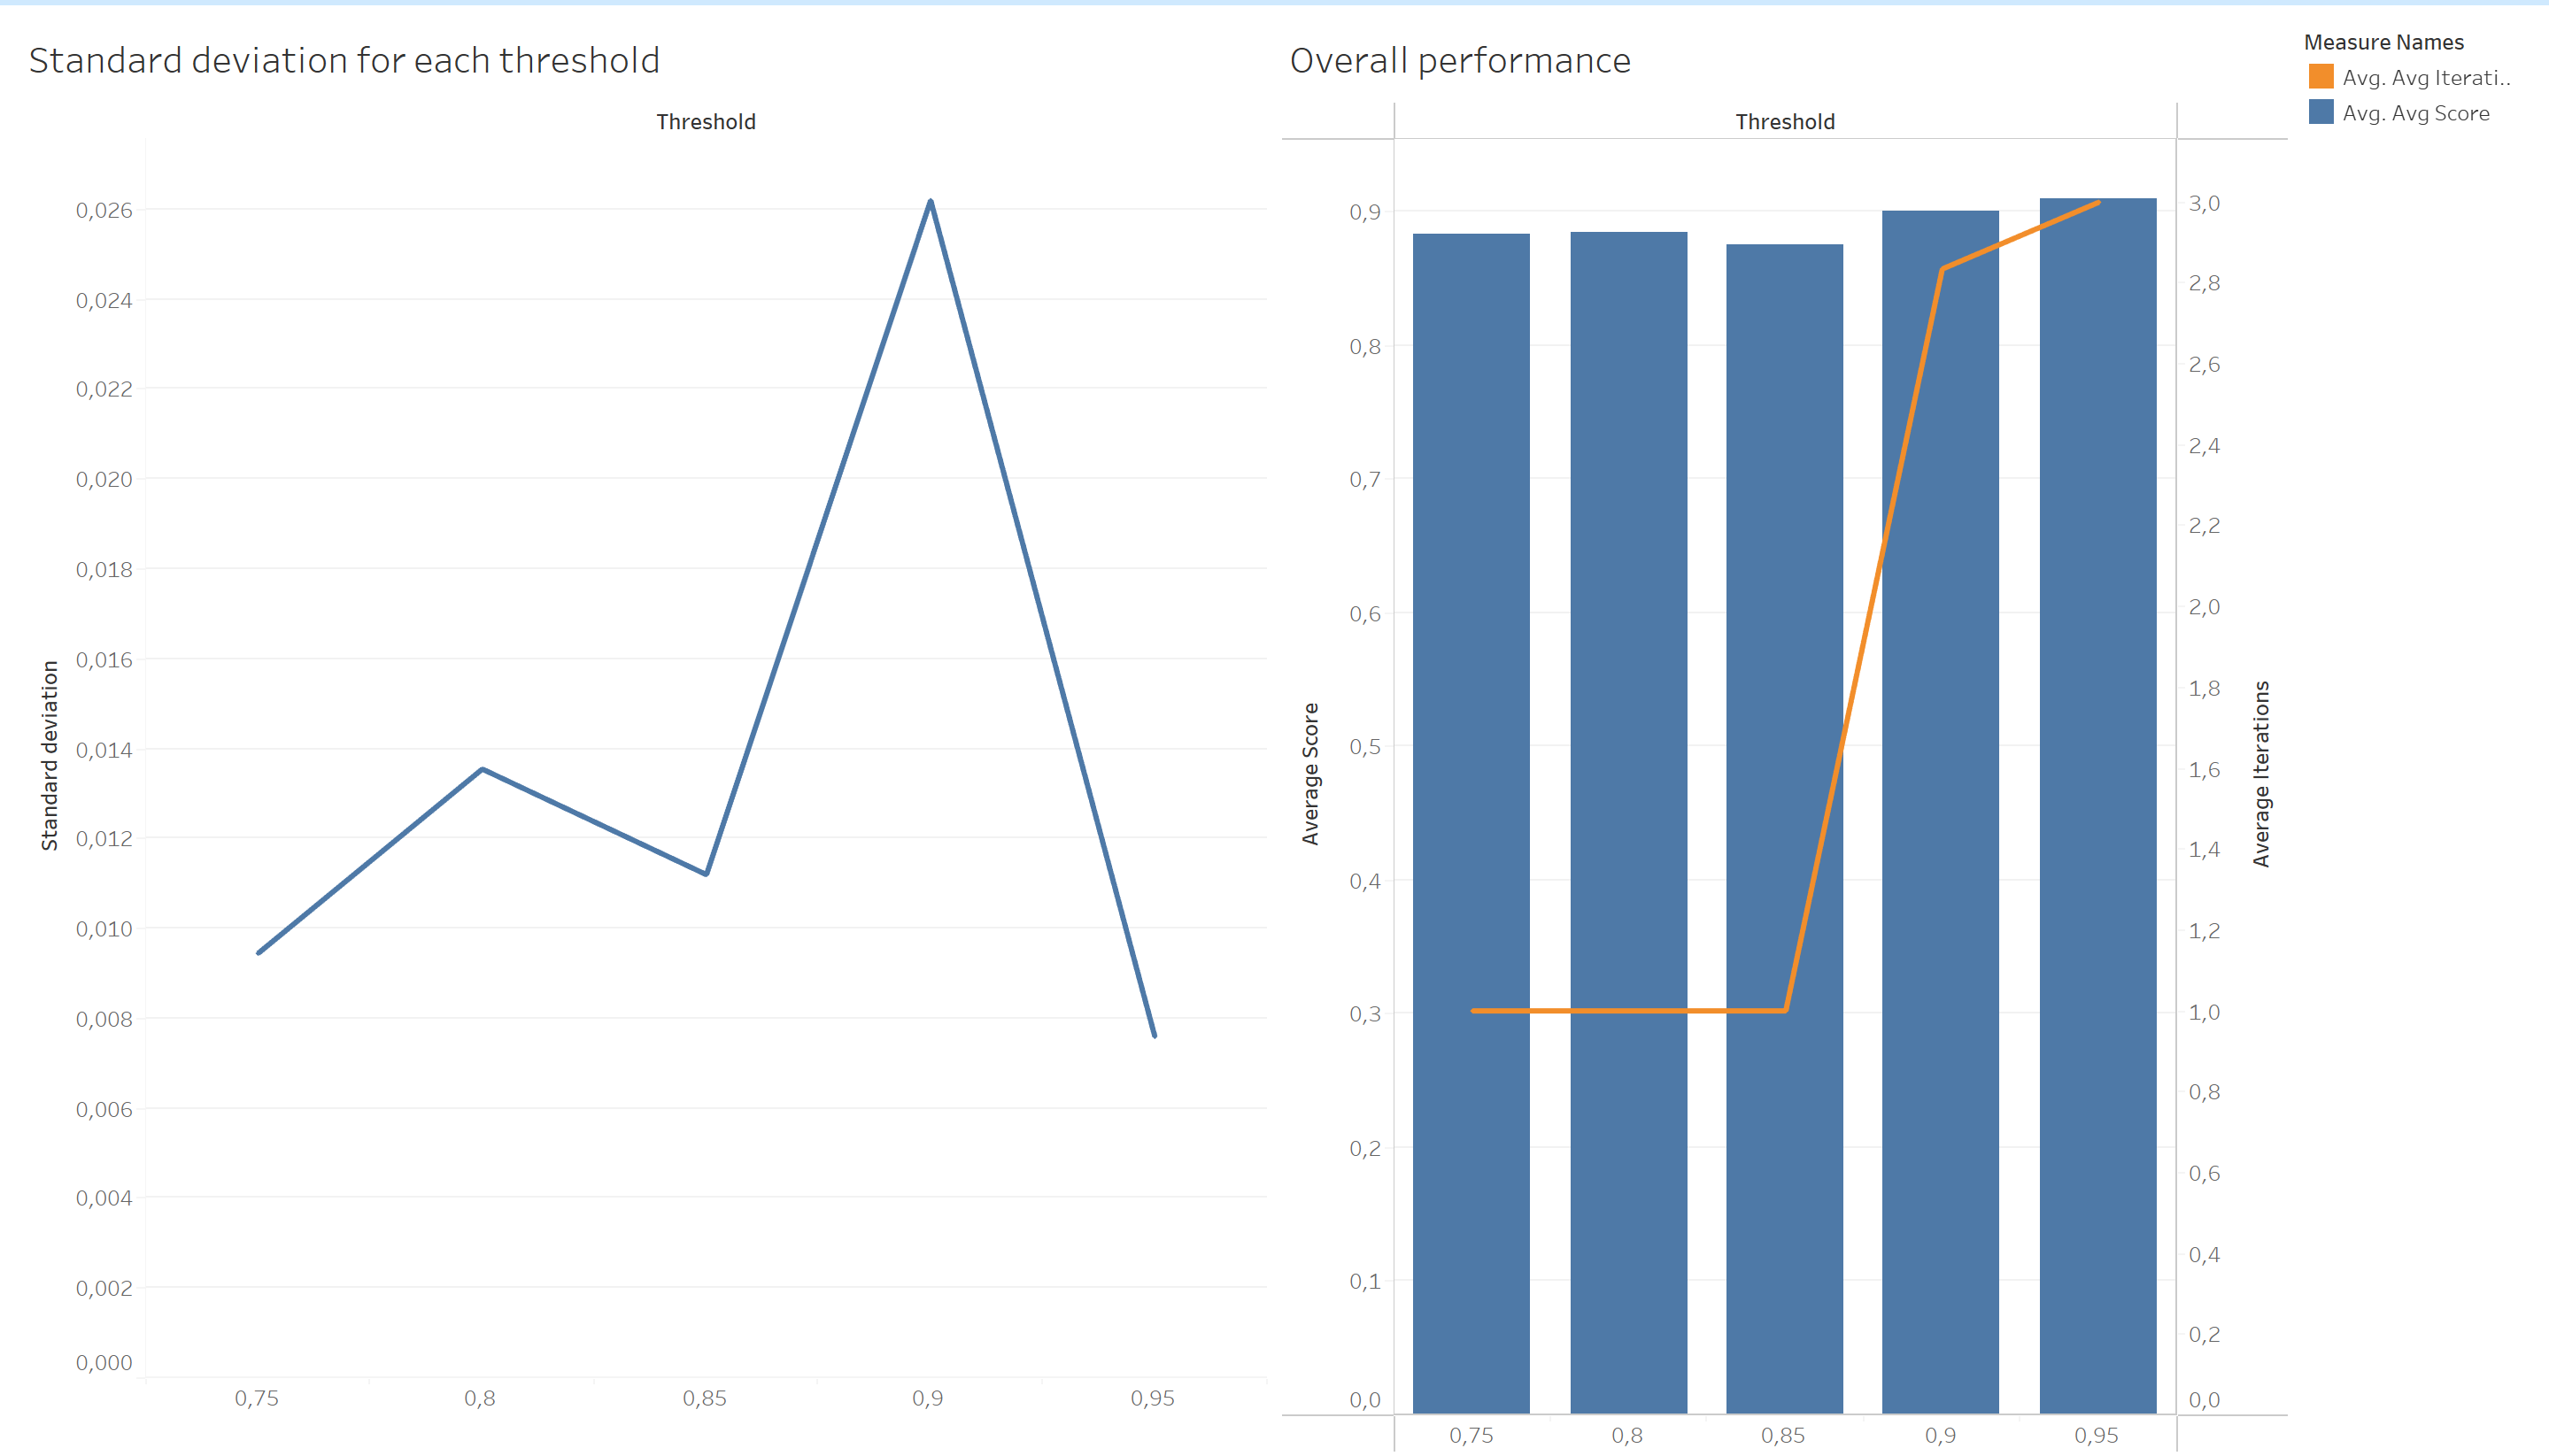
\includegraphics[width=\linewidth]{Chapters/Figures/thresholdTest.png} % Adjust width or use height
    \caption{ Threshold hold test. The blue bars represent the \textbf{Average Score} (left axis), 
while the orange line represents the \textbf{Average Number of Iterations} (right axis).  }
    \label{fig:thresholdTest}
\end{figure}

\subsection{Results and Discussion}

The self-improvement pipeline was executed on the same system description used in the previous experiments.  
After a single iteration the score grew from \(\mathbf{0.815}\) to \(\mathbf{0.855}\).

Figures~\ref{fig:SelfImprovementLoop}\,(a) and (b) show, respectively, the diagram produced in the first pass and the diagram obtained after one refinement cycle.  
While the initial model already contained the eight core domain classes, their relationships and every public operation required by the ground-truth reference, the refinement step enriched the artefact in several important ways that are directly visible when the two diagrams are compared, that goes beyond what is expressed in the system description:

\begin{itemize}
  \item \textbf{New domain concept.}  
        A dedicated TeamMember class now appears, linked to Team through a composition (\(1\;\texttt{Team}\;{\,\dashrightarrow}\;1..*\;\texttt{TeamMember}\)).  
        This makes individual contributors first-class citizens of the model.
  \item \textbf{Richer team management behaviour.}  
        The Team class gained a name attribute together with membership-handling services (\texttt{addMember}, \texttt{removeMember}, \texttt{getMembers}).  
        Complementarily, ProjectManager now offers \texttt{assignTeam(Project,\,Team)}, and TeamMember provides assignToTeam, removeFromTeam and addSkill.
  \item \textbf{Explicit traceability between artefacts and validation.}  
        WorkProduct now maintains a collection \texttt{validations: List<Validation>} and is connected to Validation through an association labelled \emph{validated by} with cardinalities \(1\leftrightarrow 0..*\).  
        Corresponding operations (\texttt{addValidation}, \texttt{getValidations}) were also added.
  \item \textbf{Refined requirement compliance.}  
        A new association \emph{validates against} relates System to one or more Requirement instances (\(1\leftrightarrow 1..*\)), turning the previously implicit link embodied in testAgainstRequirements into an explicit structural dependency.
  \item \textbf{Enhanced project coordination.}  
        The Project class is now able to register requirements and the target system by means of the newly introduced operations addRequirement and setSystem.
  \item \textbf{Extended validation feedback.}  
        Validation itself now exposes accessor methods getValidationResult and getValidationDate, providing programmatic access to the outcome and time-stamp of the validation activity.
\end{itemize}

Overall, the iteration increased the number of associations, attributes and operations, thereby improving model completeness without sacrificing correctness: no previously correct element was removed or altered erroneously.  
Although the quality when compared to the ground truth did not increased, there is an increase on the details which is important for following ativities after modelling.

\begin{figure}[htbp]
    \centering
    \subfloat[Initial diagram]{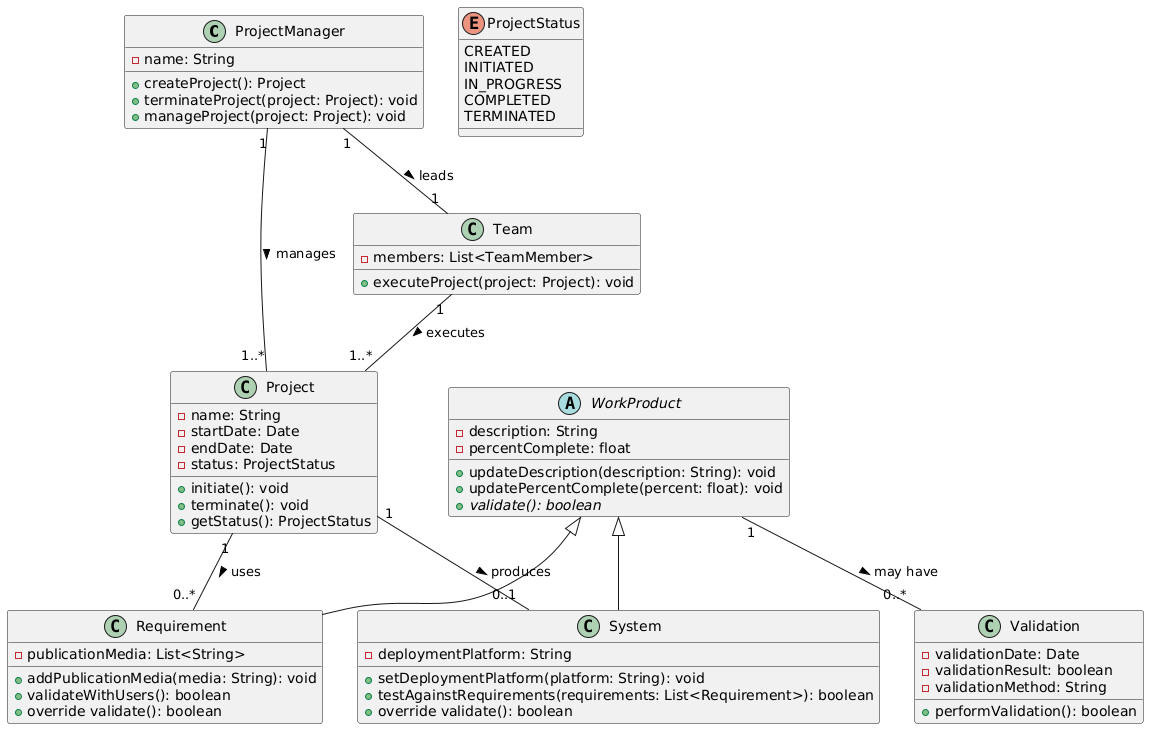
\includegraphics[width=0.45\linewidth]{Chapters/Figures/SelfImprovementGeneration.png}}
    \hfill
    \subfloat[Diagram after one self-improvement iteration]{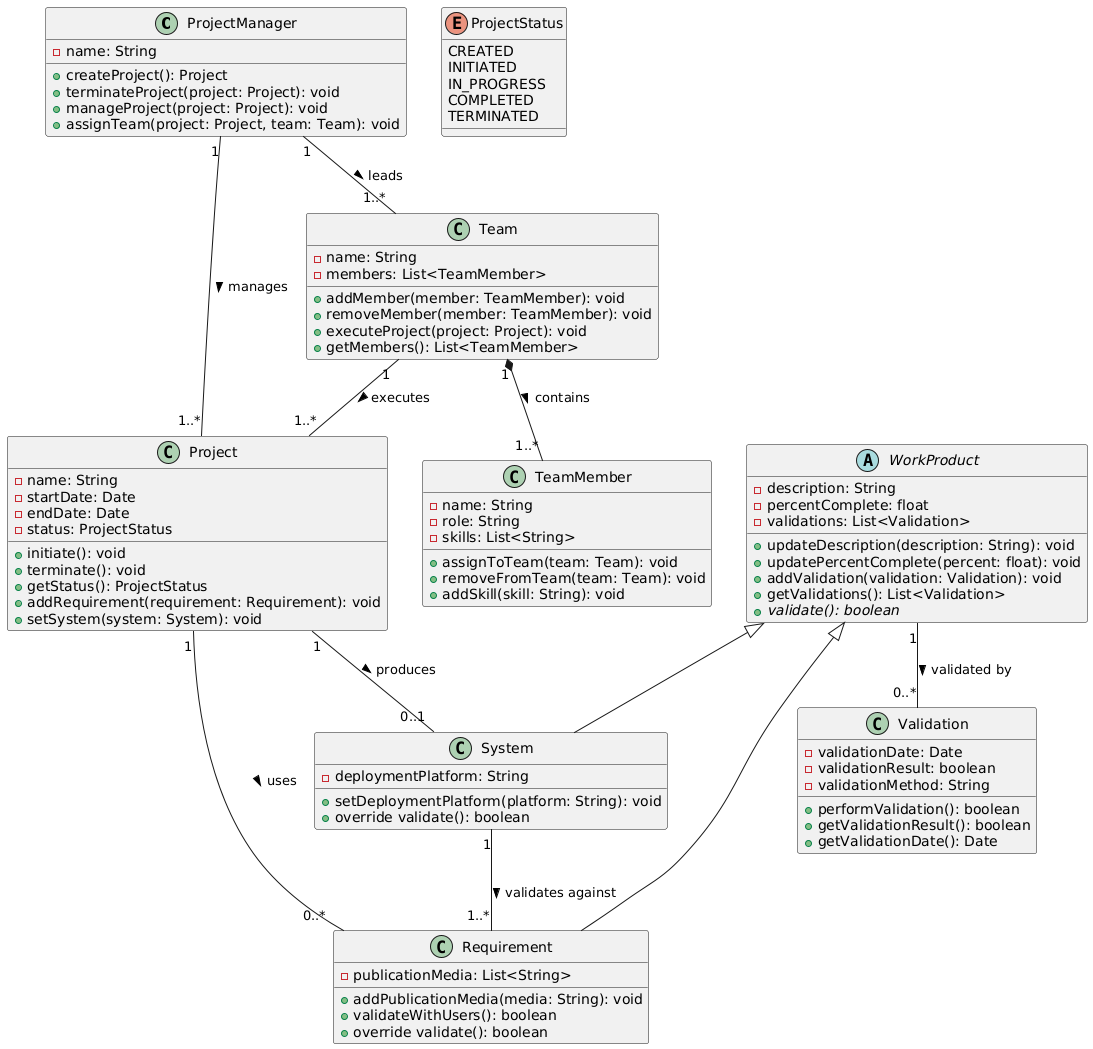
\includegraphics[width=0.45\linewidth]{Chapters/Figures/SelfImproveIteration.png}}
    \caption{Effect of the self-improvement loop on the class diagram}
    \label{fig:SelfImprovementLoop}
\end{figure}



\section{Summary}
This chapter presents a comparative study of techniques for generating UML class diagrams from natural language system descriptions using large language models (LLMs). The experiments systematically evaluate the impact of different prompt strategies (zero-shot, few-shot, and chain-of-thought) and model choices (ChatGPT-4o, Claude Sonnet 4, Deepshek XL, Gemini 2.5 Flash, and Grok 1.5) based on structural, semantic, and lexical criteria. 
% Concise lead-in + results in structured bullet points
The main findings from the experiments are summarised below:

\begin{itemize}
    \item \textbf{Prompt strategies}
    \begin{itemize}
        \item Chain-of-thought prompting improved recall and semantic coverage, particularly for low-salience elements.
        \item Few-shot prompting achieved the highest ROUGE scores, indicating stronger lexical alignment.
    \end{itemize}

    \item \textbf{Model comparison}
    \begin{itemize}
        \item Claude Sonnet 4 was the most balanced model in terms of structural and semantic performance.
        \item Open-source models were excluded from further analysis due to weak results and practical constraints.
    \end{itemize}

    \item \textbf{Retrieval-Augmented Generation (RAG)}
    \begin{itemize}
        \item In NotebookLM, an adapted zero-shot prompt that leveraged document-grounded context produced diagrams closest to the ground truth, outperforming both standard zero-shot and few-shot setups.
    \end{itemize}

    \item \textbf{Self-refinement (Claude + Self-Refine)}
    \begin{itemize}
        \item The system autonomously generated, critiqued, and iteratively refined its UML output until a predefined quality threshold was met.
        \item This process increased completeness and detail—adding relevant classes and relationships—without reducing correctness.
        \item Threshold testing indicated that a target score of \textbf{0.85} offered the best trade-off between quality and efficiency.
    \end{itemize}
\end{itemize}

Our approach pretend to be, the combination of prompt engineering, document grounding, and self-refinement which provides a low-cost, effective strategy for improving the quality of UML diagram generation in resource-constrained environments.